% -------------------------------------------------------------------------------- %

\begin{exercise}

Berechnen Sie die Ableitung der Funktion

\begin{align*}
    f(t)
    =
    \Int[0][1]
    {
        \frac{1}{x}
        \sin(t x)
    }{x}.
\end{align*}

Begründen Sie dabei genau alle nichtelementaren Schritte!

\end{exercise}

% -------------------------------------------------------------------------------- %

\begin{solution}

\phantom{}

\begin{align*}
    g(t, x)
    =
    \frac{1}{x}
    \sin(t x)
    \implies
    \lim_{x \to 0}
    g(t, x)
    =
    \lim_{x \to 0}
    \frac{\sin(t x) - \sin{0}}{x - 0}
    =
    \pderivative{x}
    \sin(t x)
    \Big |_{x=0}
    =
    t \cos(t 0)
    =
    t
\end{align*}

Wir können also den Integranden $g$ stetig auf ganz $[0, 1]^2$ fortsetzen.

\begin{tcolorbox}[standard jigsaw, opacityback = 0]
    \centering
    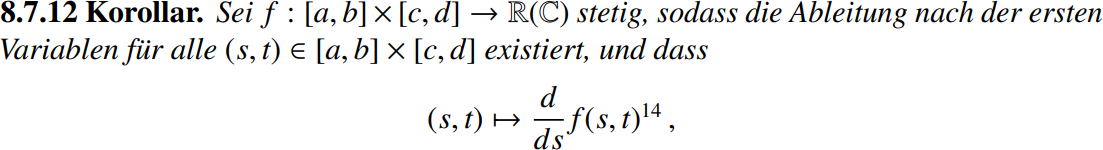
\includegraphics
    [width = 0.75 \textwidth]
    {Ana1&2/Ana1&2 - 8.7.12.1 Korollar.png} \\
    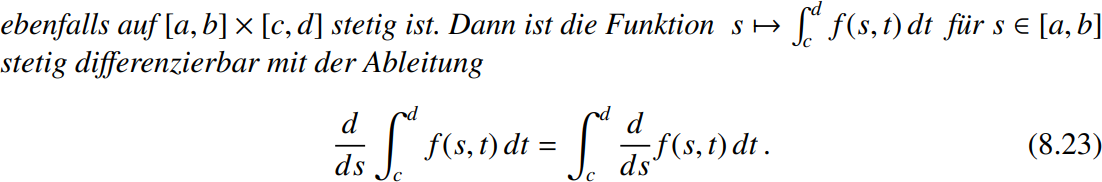
\includegraphics
    [width = 0.75 \textwidth]
    {Ana1&2/Ana1&2 - 8.7.12.2 Korollar.png}
\end{tcolorbox}

Laut Korollar 8.7.12, können wir also die Ableitung in das Parameterintegral hineinziehen.

\begin{align*}
    \implies
    f^\prime(t)
    =
    \Int[0][1]
    {
        \derivative{t}
        \frac{1}{x}
        \sin(t x)
    }{x}
    =
    \Int[0][1]
    {
        \cos(t x)
    }{x}
    \stackrel{!}{=}
    \frac{1}{t}
    \Int[0][t]{\cos u}{u}
    =
    \frac{1}{t}
    \sin{u} \Big |_{u=0}^t
    =
    \frac{\sin t}{t}
\end{align*}

Dabei haben wir folgende Substitution verwendet.

\begin{align*}
    u = t x
    \implies
    \derivative[][u]{x} = t
    \implies
    \mathrm{d}x = \mathrm{d}u \frac{1}{t}
\end{align*}

\end{solution}

% -------------------------------------------------------------------------------- %
